% TODO
% Black body radiation


\section{Thermal Physics}
    \subsection{Heat transmition}
        Three ways of heat transmition:
        \begin{enumerate}
            \item Conduction
            \item Radiation
            \item Convection
        \end{enumerate}

        \paragraph{Conduction}
            This way need media.
            Fourier's law: as shown in Figure \ref{}, the rate of heat transfer is
            \begin{align}
                \frac{\mathrm{d} Q}{\mathrm{d} t} = -\frac{A}{k} \frac{\mathrm{d} T}{\mathrm{d} l}
            \end{align}

            There is negative because the high-temperature end (which means $\mathrm{d} t > 0$) lose energy (which means $\mathrm{d} Q < 0$).
        
        \paragraph{Convection}
            Newton cooling law: 
            \begin{align}
                \frac{\mathrm{d} T}{\mathrm{d} t} \propto \Delta T
            \end{align}
            Temperature change rate is propotional to temperature difference.

        \paragraph{Radiation}
            This way does not need media. Energy transfered in form of EM wave.

            Albedo rate:
            \begin{align}
                a = \frac{P_{\mathrm{out}}}{P_{\mathrm{in}}}
            \end{align}

    \subsection{Ideal gas}
        \paragraph{Properties}
            \begin{enumerate}
                \item Gas molecules are point particles.
                \item Molecules follow laws of mechanism.
                \item Only collision force exist among molecules.
                \item Collisions are elastic which means no energy loss.
                \item Molecules move totally random.
                \item Cannot be solidify or liquidify due to temperature and pressure change.
            \end{enumerate}
        
        \paragraph{Ideal gas equation}
            \begin{align}
                P V = \gamma R T
            \end{align}
            $P$ is pressure, $V$ is volumn, $\gamma$ is number of moles of the gas, $R$ is gas constant, $T$ is temperature. $R \approx 8.31$.

            Boltzmann constant, $k_B$, is defined as 
            \begin{align}
                k_B = \frac{R}{N_A}
            \end{align}

        \paragraph{Isothermal process}
            Temperature is constant. The internal energy of gas stay same. $P \propto \frac{1}{V}$.

        \paragraph{Isobanic process}
            Pressure is constant. $V \propto T$.
            
        \paragraph{Isovolumn process}
            Volumn is constant. $P \propto T$.

        \paragraph{Pressure of gas}
            Pressure is caused by gas molecules continously hitting on the wall of container. As shown in Figure \ref{hit_wall}, the velocity of the molecule is $v$ and mass is $m$.

            \begin{figure}[H]
                \begin{center}
                    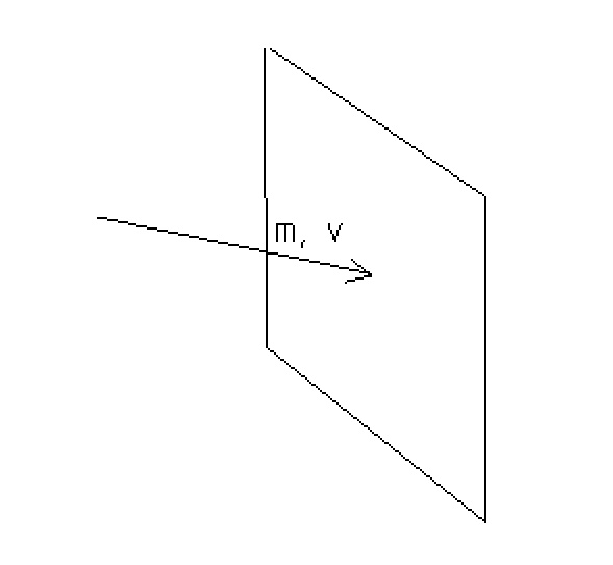
\includegraphics[height=4cm]{thermal_charts/hit_wall.eps}
                \end{center}
                \caption{Gas molecules collide on wall of container}
                \label{hit_wall}
            \end{figure}

            In small cube with side length $d$ as shown in Figure \ref{small_cub_hit}, the time for one collide on a wall is
            \begin{align}
                t = \frac{2d}{v}
            \end{align}

            \begin{figure}[H]
                \begin{center}
                    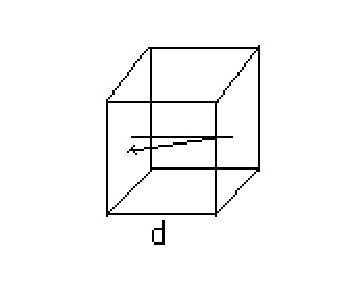
\includegraphics[height=3cm]{thermal_charts/small_cube_collide.eps}
                \end{center}
                \caption{Time for one collide in small cube}
                \label{small_cub_hit}
            \end{figure}

            Thus, the average force on that wall is
            \begin{align}
                F &= \frac{\Delta p}{t} \\
                  &= \frac{2 m v_x}{\frac{2 d}{v_x}} \\
                  &= \frac{m {v_x}^2}{d}
            \end{align}

            Here, $v_x$ is the component of velocity perpendicular to the wall. Since it is randomly three-dimension motion, velocity component in each of three direction is same. Thus
            \begin{align}
                \left\{
                    \begin{aligned}
                        & {v_x}^2 + {v_y}^2 + {v_z}^2 = v^2 \\
                        & v_x = v_y = v_z
                    \end{aligned}
                \right. \Rightarrow
                {v_x}^2 = \frac{1}{3} v^2
            \end{align}

            \begin{align}
                F = \frac{m v^2}{3 d}
            \end{align}

            Thus, the pressure is
            \begin{align}
                P &= \frac{F}{A} \\
                  &= \frac{\frac{m v^2}{3 d}}{d^2} \\
                  &= \frac{m v^2}{3 d^3} \\
                  &= \frac{1}{3} \rho v^2
            \end{align}




        \paragraph{Energy of molecule}
            Total internal energy = Potential energy + Kinetic energy. In ideal gas model, there is no potential energy.

            Energy of all molecules is
            \begin{align}
                & P = \frac{m v^2}{3 d^3} = \frac{\gamma R T}{V} \\
                & \Rightarrow m v^2 = 3 \gamma R T \\
                & \Rightarrow E = \frac{1}{2} m v^2 = \frac{3}{2} \gamma R T
            \end{align}

            Energy of a single molecule is
            \begin{align}
                E_i &= \frac{E}{\gamma N_A} \\
                    &= \frac{3 R T}{2 N_A}
            \end{align}

    \subsection{Black body radiation}
        \paragraph{Stefan-Boltzmann law}
            \begin{align}
                P = \sigma A T^4
            \end{align}

            $P$: radiate power; $A$: cross-area; $\sigma$: Stefan-Boltzmann constant; $T$: temperature.

        \paragraph{Wien's displacement law}
            \begin{align}
                \lambda_{\mathrm{max}} T &= b \\
                                       b &= 2.9 \times 10^{-3}
            \end{align}

            $\lambda_{\mathrm{max}}$: Wave length in which radiate intensity is the maximum; $b$: Wien's displacement constant; $T$: temperature.

        \paragraph{Emissivity}
            $e$, Ratio of power emitted by an object to power emitted by black body with same dimension and temperature.

            For real objects, radiate power
            \begin{align}
                P = e \sigma A T^4
            \end{align}